\chapter{Caracter\'isticas de la fotograf\'ia de desnudo.}

\section{\textquestiondown Q\'ue entendemos por fotograf\'ia de desnudo?}
Tal y como se expresa en la Wikipedia\cite{wiki:xxx} el desnudo es g\'enero art\'istico que consiste en la representaci\'on en los medios art\'isticos del cuerpo humano desnudo, siendo una de las clasificaciones de las obras de arte.

Tras la aparici\'on de la fotograf\'ia

El empleo de una dist\'ancia focal adecuada, para la que tendremos que tener en cuenta el  \gls{angulovision} asociado tal y como se puede ver en la tabla asociada\ref{fig:angulos2-1}.

\begin{figure}[th!]
	\centering
	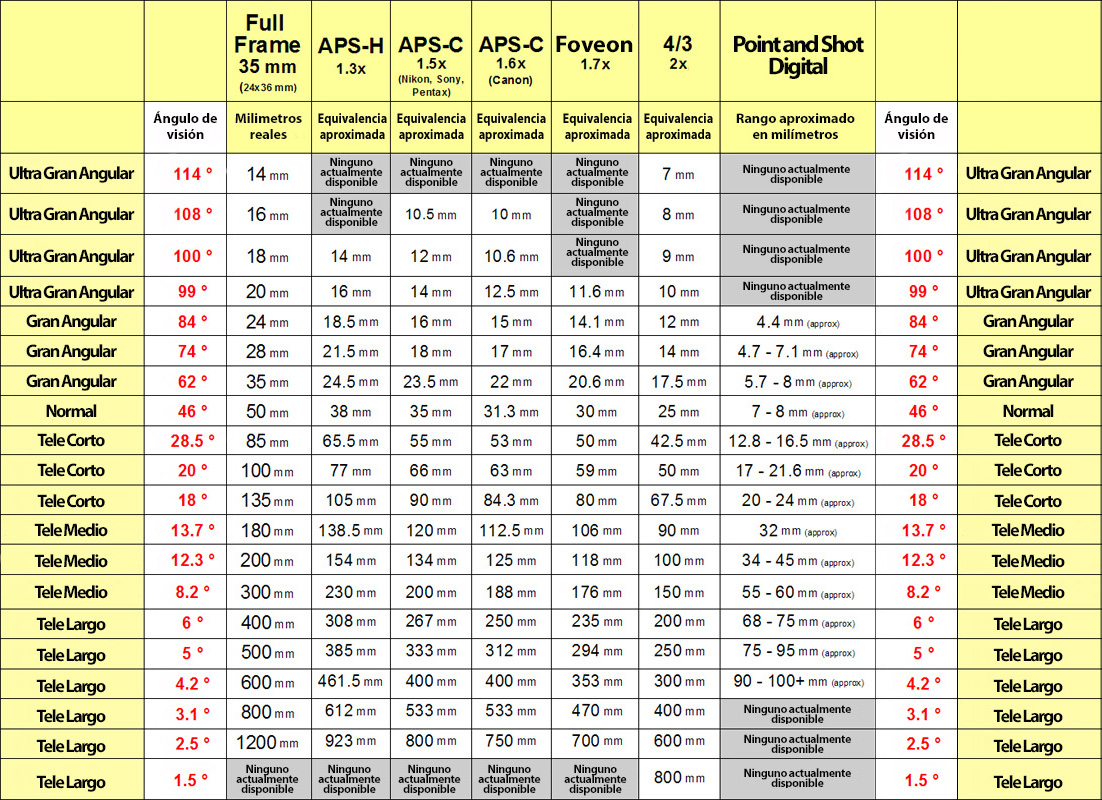
\includegraphics[width=0.7\linewidth]{imagenes/angulos2-1}
	\caption[Resumen de formatos, distancias focales y \'angulos en lentes]{Resumen y tabla de conversi\'on de distancias focales en funci\'on de los sensores que se est\'en empleando\cite{web:estudionadjar}.}
	\label{fig:angulos2-1}
\end{figure}
